\chapter{Chip Characterization}

After the chip was fabricated, characterizations were done on each sensor site to determine the best shape, size, pitch, and organization of the electrodes. This was done using differential pulse voltammetry (DPV). DPV is a technique similar to cyclic voltammetry (CV), but which is better because [TODO]. A CH Instruments 660B was used to perform all of the following tests.

The method used was to test two random sensors on each of the 21 sensor sites with 3 tests on each sensor, thus 6 tests on each sensor site. A cleaning was done on each sensor before testing using CV from 1.0V to -0.3V at 1V/s and 20 cycles with $\mathrm{H_2SO_4}$. Tests were performed with DPV from -0.2V to 0.2V with 0.3mM norepinephrine in 0.1M $\mathrm{H_2SO_4}$. A peak formed at around 0.0V. The amplitude of the highest part of the peak in relation to the average baseline (the straight line between the beginning and end of the peak) was taken as the value of a test. Results were compiled by averaging all six tests from each sensor site (Table \ref{DPV results}).

\begin{table}
	\begin{tabular}{lll}
		Sensor & \% of max & Avg. value \\
		\hline
		17 & 100.0 $\pm$ 4.0 & 7.04e-10 $\pm$ 2.83e-11 \\
		8 & 77.9 $\pm$ 5.5 & 5.48e-10 $\pm$ 3.85e-11 \\
		16 & 75.7 $\pm$ 1.8 & 5.32e-10 $\pm$ 1.28e-11 \\
		7 & 71.5 $\pm$ 3.0 & 5.03e-10 $\pm$ 2.13e-11 \\
		18 & 58.8 $\pm$ 2.5 & 4.14e-10 $\pm$ 1.73e-11 \\
		6 & 57.6 $\pm$ 4.0 & 4.05e-10 $\pm$ 2.79e-11 \\
		15 & 55.2 $\pm$ 3.5 & 3.89e-10 $\pm$ 2.43e-11 \\
		14 & 50.8 $\pm$ 2.1 & 3.57e-10 $\pm$ 1.46e-11 \\
		10 & 47.6 $\pm$ 3.6 & 3.35e-10 $\pm$ 2.50e-11 \\
		5 & 43.0 $\pm$ 1.2 & 3.03e-10 $\pm$ 8.27e-12 \\
		1 & 36.7 $\pm$ 3.5 & 2.58e-10 $\pm$ 2.46e-11 \\
		20 & 26.1 $\pm$ 1.0 & 1.84e-10 $\pm$ 7.29e-12 \\
		0 & 23.8 $\pm$ 5.0 & 1.68e-10 $\pm$ 3.55e-11 \\
		19 & 21.9 $\pm$ 2.0 & 1.54e-10 $\pm$ 1.44e-11 \\
		12 & 19.5 $\pm$ 1.5 & 1.37e-10 $\pm$ 1.05e-11 \\
		4 & 19.2 $\pm$ 1.8 & 1.35e-10 $\pm$ 1.28e-11 \\
		13 & 19.1 $\pm$ 1.0 & 1.34e-10 $\pm$ 7.37e-12 \\
		2 & 17.6 $\pm$ 2.1 & 1.24e-10 $\pm$ 1.49e-11 \\
		9 & 17.5 $\pm$ 0.4 & 1.23e-10 $\pm$ 2.83e-12 \\
		11 & 14.4 $\pm$ 1.9 & 1.01e-10 $\pm$ 1.33e-11 \\
		3 & 11.3 $\pm$ 1.3 & 7.93e-11 $\pm$ 9.48e-12
	\end{tabular}
	\caption[DPV results for sensor sites]{DPV results for sensor sites sorted by decreasing value}
	\label{DPV results}
\end{table}

Sensor sites 17 and 8 had the best results. Since those sensors have different electrode configuration [TODO: discuss electrode configuration, shape, etc.], testing was done on both sensors to determine the lowest detectable concentration using the same DPV procedure as above, but with decreasing concentrations of norepinephrine starting at 0.3mM and decreasing by a factor of 3 each iteration (Figure \ref{limit figure}). Sensor 17 (Table \ref{limit 17}) was able to detect down to about 3$\mu$M with a linear fit of $A = 1.88996e-6 * M - 2.36855e-12$, where $A$ is the resulting current in amperes and $M$ is the concentration molarity. Sensor 8 (Table \ref{limit 8}) was able to detect down to about 10$\mu$M with a linear fit of $A = 8.29117e-7 * M + 4.3417e-11$, where $A$ is the resulting current in amperes and $M$ is the concentration molarity.


\begin{table}
	\begin{tabular}{ll}
		Concentration (M) & Peak value \\
		\hline
		0.0003 & 5.609E-10 \\
		0.0003 & 5.591E-10 \\
		0.0001 & 1.988E-10 \\
		0.0001 & 2.082E-10 \\
		0.000033 & 5.701E-11 \\
		0.000033 & 4.788E-11 \\
		0.000011 & 1.306E-11 \\
		0.000011 & 1.439E-11 \\
	\end{tabular}
	\caption[Detection limit results for sensor 17]{Detection limit results for sensor 17 sorted by decreasing concentration}
	\label{limit 17}
\end{table}

\begin{table}
	\begin{tabular}{ll}
		Concentration (M) & Peak value \\
		\hline
		0.0003 & 2.926E-10 \\
		0.0003 & 2.663E-10 \\
		0.0001 & 1.786E-10 \\
		0.0001 & 1.753E-10 \\
		0.000033 & 3.276E-11 \\
		0.000033 & 3.296E-11 \\
	\end{tabular}
	\caption[Detection limit results for sensor 8]{Detection limit results for sensor 8 sorted by decreasing concentration}
	\label{limit 8}
\end{table}

\begin{figure}
\centering
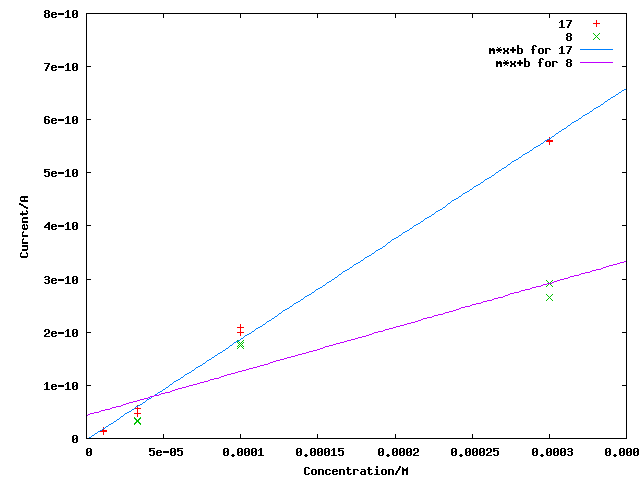
\includegraphics[width=\linewidth]{figures/limit.png}
\caption{Detection limits}
\label{limit figure}
\end{figure}
